% !TeX root = ../main.tex

\chapter{实验及结果分析}

\section{实验设计}

为验证本文所述模型的有效性,本文作者进行了如下实验:

1. 使用 Y 编译器内置的耗时预测模型,即类似第二章第二节所述的传统方法进行耗时预测,该实验结果作为 baseline。

2. 不使用图神经网络聚合结点之间的嵌入向量,将边上的张量特征编码到它的头节点上,仅使用全连接神经网络获得各个结点的嵌入向量。

3. 使用只能处理结点特征的图神经网络,将边上的张量特征编码到它的头节点上。

4. 使用能处理边特征的图神经网络,即本文模型。

5. 在本文模型的基础上,不使用全连接神经网络获取低维嵌入,将结点和边的特征直接作为图神经网络的输入。

\section{实验结果与分析}

本文按照 8 : 1 : 1 的比例划分训练集、验证集和测试集,同时控制 batch\_size 为 512,学习率为 0.001。
为防止过拟合,本文采用早停法 \cite{earlystop} 进行训练,当验证集上的肯德尔秩相关系数连续 40 次迭代
没有超过最大值时,停止训练并计算测试集的各项指标。

实验结果如表 \ref{tab:table3}, 图 \ref{fig:graph9} 和图 \ref{fig:graph10} 所示:

\begin{table}[]
    \centering
    \caption{实验结果}
    \begin{threeparttable}
        \scalebox{0.55}{
            \begin{tabular}{|c|ccc|ccc|ccc|ccc|c|}
                \hline
                \multirow{2}{*}{实验/指标} & \multicolumn{3}{c|}{MAE}                                                                & \multicolumn{3}{c|}{MAPE}                                                                     & \multicolumn{3}{c|}{肯德尔秩相关系数}                                                                       & \multicolumn{3}{c|}{每个 IR 的肯德尔秩相关系数}                                                                & 训练轮数         \\ \cline{2-14} 
                                       & \multicolumn{1}{c|}{训练集}           & \multicolumn{1}{c|}{验证集}           & 测试集           & \multicolumn{1}{c|}{训练集}             & \multicolumn{1}{c|}{验证集}             & 测试集             & \multicolumn{1}{c|}{训练集}               & \multicolumn{1}{c|}{验证集}               & 测试集               & \multicolumn{1}{c|}{训练集}               & \multicolumn{1}{c|}{验证集}               & 测试集               &              \\ \hline
                传统方法\tnote{a}           & \multicolumn{1}{c|}{3157.91}       & \multicolumn{1}{c|}{3231.32}       & 2635.91       & \multicolumn{1}{c|}{694.71\%}        & \multicolumn{1}{c|}{683.14\%}        & 643.57\%        & \multicolumn{1}{c|}{0.849991}          & \multicolumn{1}{c|}{0.855742}          & 0.856881          & \multicolumn{1}{c|}{0.483465}          & \multicolumn{1}{c|}{0.486368}          & 0.493708          & /            \\ \hline
                全连接神经网络              & \multicolumn{1}{c|}{32.22}         & \multicolumn{1}{c|}{34.23}         & 34.32         & \multicolumn{1}{c|}{17.83\%}         & \multicolumn{1}{c|}{19.39\%}         & 18.84\%         & \multicolumn{1}{c|}{0.886773}          & \multicolumn{1}{c|}{0.882635}          & 0.880815          & \multicolumn{1}{c|}{0.602722}          & \multicolumn{1}{c|}{0.586192}          & 0.588023          & 571          \\ \hline
                仅使用结点特征              & \multicolumn{1}{c|}{8.43}          & \multicolumn{1}{c|}{13.47}         & 10.72         & \multicolumn{1}{c|}{3.73\%}          & \multicolumn{1}{c|}{5.51\%}          & 4.52\%          & \multicolumn{1}{c|}{0.972270}          & \multicolumn{1}{c|}{0.958332}          & 0.966824          & \multicolumn{1}{c|}{0.828374}          & \multicolumn{1}{c|}{0.798427}          & 0.812764          & 444          \\ \hline
                本文模型                    & \multicolumn{1}{c|}{\textbf{4.46}} & \multicolumn{1}{c|}{\textbf{8.01}} & \textbf{6.13} & \multicolumn{1}{c|}{\textbf{1.87\%}} & \multicolumn{1}{c|}{\textbf{2.63\%}} & \textbf{2.40\%} & \multicolumn{1}{c|}{\textbf{0.987974}} & \multicolumn{1}{c|}{\textbf{0.982281}} & \textbf{0.984161} & \multicolumn{1}{c|}{\textbf{0.861613}} & \multicolumn{1}{c|}{\textbf{0.845762}} & \textbf{0.839584} & \textbf{300} \\ \hline
                不使用全连接层              & \multicolumn{1}{c|}{5.26}          & \multicolumn{1}{c|}{8.24}          & 6.96          & \multicolumn{1}{c|}{2.03\%}          & \multicolumn{1}{c|}{2.79\%}          & 2.61\%          & \multicolumn{1}{c|}{0.987702}          & \multicolumn{1}{c|}{0.981660}          & 0.983421          & \multicolumn{1}{c|}{0.856425}          & \multicolumn{1}{c|}{0.838511}          & 0.835196          & 368          \\ \hline
                \end{tabular}}
                \begin{tablenotes}
                    \footnotesize
                    \item[a] 传统方法主要关注计算图运行时间的相对大小,故在 MAE 和 MAPE 上和其他方法存在数量级的差异。
                \end{tablenotes}
    \end{threeparttable}

    \label{tab:table3}
\end{table}



\begin{figure}[H]
    \centering
    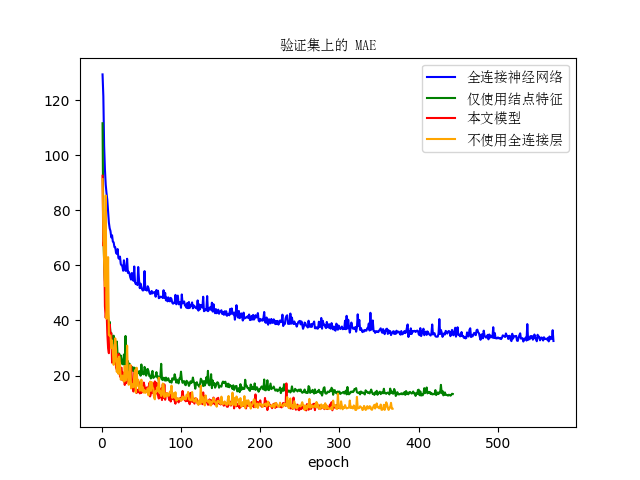
\includegraphics[scale=0.8]{figures/mae.png}
    \caption{验证集上的 MAE}
    \label{fig:graph9}
\end{figure}

\begin{figure}[htp]\scriptsize
    \begin{center}
    \subfigure[整体的肯德尔秩相关系数]{
        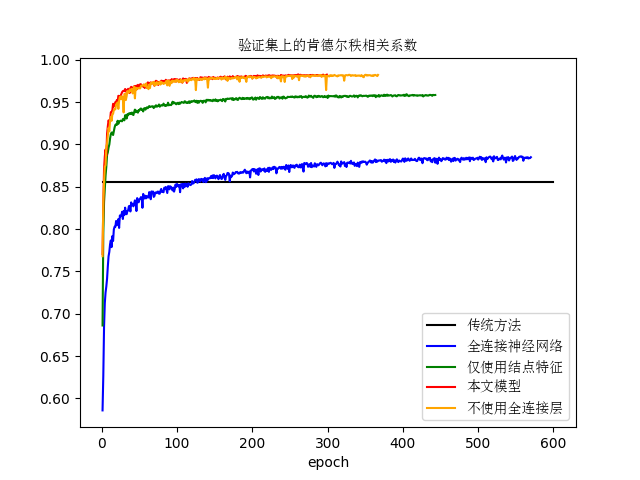
\includegraphics[width=0.47\textwidth]{figures/tau.png}}
    \subfigure[每个 IR 的肯德尔秩相关系数]{
        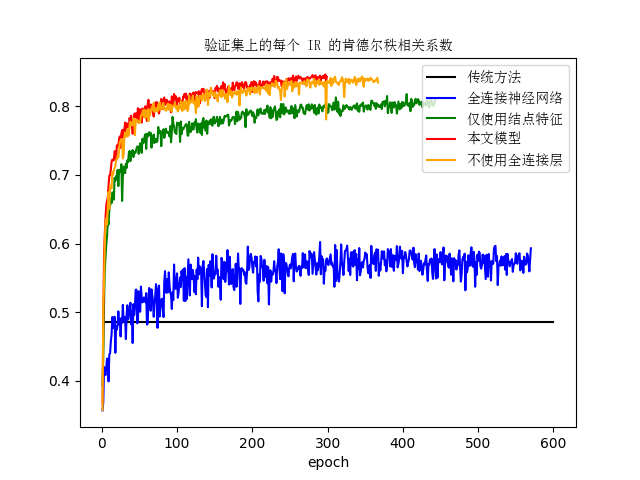
\includegraphics[width=0.47\textwidth]{figures/ir_tau.png}}
    \caption{验证集上的肯德尔秩相关系数}
    \label{fig:graph10}
    \end{center}
\end{figure}

由上述实验结果可以得到以下结论:

1. 对比表 \ref{tab:table3} 第一行和第二行,发现仅使用两层全连接神经网络即可达到超过传统方法的预测效果,说明在处理计算图耗时预测这样的复杂问题上,简单的全连接神经网络就可以超过人类专家。

2. 对比表 \ref{tab:table3} 第二行和第三行,发现相比于简单的全连接神经网络,使用图神经网络进行计算图耗时预测会得到更准确的结果。在分别以 MAPE 和肯德尔秩相关系数作为评价标准的前提下,使用图神经网络相较于仅使用全连接神经网络均得到相对显著的提升。
观察图 \ref{fig:graph9} 和图 \ref{fig:graph10},可以发现图神经网络方法可以在训练更少次数的前提下达到收敛。尤其通过图 \ref{fig:graph10}(b) 可以发现,相比于全连接神经网络,图神经网络方法的平均每个 IR 的肯德尔秩相关系数的震荡幅度更小,说明图神经网络方法的模型更加稳定。

3. 对比表 \ref{tab:table3} 第三行和第四行,发现相比于将计算图边上的张量特征编码到边的头结点上,使用能够处理边特征的图神经网络可以使预测结果得到较为明显的提升,充分说明了将张量特征编码到图神经网络的边上是更为合理的建模方式。

4. 对比表 \ref{tab:table3} 第四行和第五行,发现相比于直接将结点和边的特征向量作为图神经网络的输入,先使用全连接神经网络初步提取相关特征会使预测的效果有微小的提升。观察图 \ref{fig:graph10} 可知使用全连接层初步提取特征可以使模型更稳定。
但相比于其他因素,是否使用全连接层对于计算图耗时预测模型的影响较小,说明影响预测效果的关键在于图神经网络。

综上所述,本文提出的模型在各个评价指标上均显著优于传统方法,说明基于图神经网络的模型能够较好地完成计算图耗时预测任务。